\documentclass[a4paper,12pt]{article}
\usepackage{fancyhdr}
\setlength{\headheight}{14.49998pt}
\addtolength{\topmargin}{-2.49998pt}

% caricamento dei diversi pacchetti
\usepackage{fancyhdr}
\usepackage{graphicx}  % Per inserire le immagini
\usepackage{float}     % Per l'opzione H nei float
\usepackage{geometry}
\usepackage{lipsum}
\usepackage{hyperref}  % Per rendere l'indice cliccabile
\usepackage{enumitem}

\geometry{top=2.5cm,bottom=2.5cm,left=2.5cm,right=2.5cm}

% Intestazioni personalizzate
\pagestyle{fancy}
\fancyhf{}  % Pulisce l'intestazione e il piè di pagina
\fancyhead[C]{UniMarket}
\fancyfoot[C]{Progetto di Ingegneria del Software}
\fancyfoot[R]{\thepage}
\renewcommand{\footrulewidth}{0.4pt}
\begin{document}

% Titolo
\begin{titlepage}
    \centering
    \vspace*{2cm}
    
    \vspace{1.5cm}
    
    % Titolo del progetto
    \large Documentazione

    \Huge
    \textbf{UniMarket}
    
    \vspace{1.5cm}
    
    % Titolo del corso e altri dettagli
    \LARGE
    Progetto di Ingegneria del Software
    
    \vspace{1.5cm}
    
\includegraphics[width=0.5\textwidth]{../Media/logo.jpeg}
    
    \vspace{1.5cm}
    % Autori del progetto
    \small
    \textbf{Di Davide Dell'Anno}, \textbf{Davide Carissoni}, \textbf{Francesca Corrente}
    
    \vspace{1.5cm}
    
    % Dati dell'università
    \Large
    Università degli Studi di Bergamo 

    Facoltà di Ingegneria Informatica 

    2024-2025
    
\end{titlepage}

% Indice
\renewcommand{\contentsname}{Indice}
\tableofcontents
\newpage

\section{Project Plan}

% Capitoli e sottosezioni
\subsection{Introduzione} %fra
UniMarket è stato progettato con l'obiettivo di semplificare la gestione della spesa per gli studenti.\\  
Si tratta di un'applicazione che consente di selezionare facilmente i prodotti desiderati e creare un carrello virtuale, ottimizzando il processo di ricerca e acquisto. \\
L'applicazione non solo semplifica la gestione della spesa quotidiana, ma offre anche funzionalità pensate per le esigenze specifiche degli studenti, come la possibilità di salvare le proprie liste della spesa, monitorare i costi in tempo reale per rispettare il budget mensile e ricevere notifiche su offerte speciali o sconti. \\
UniMarket mira a migliorare l'esperienza di spesa online, offrendo una soluzione pratica ed efficiente per le esigenze quotidiane degli studenti.

\subsection{Modelli di Processo} %davide
Lo sviluppo del progetto seguirà un processo \textbf{RAD} (Rapid Application Development), con l’obiettivo di realizzare un’applicazione funzionante entro i tempi stabiliti dal \textit{time box}.  
Verrà adottato il \textbf{modello di Kano} per classificare i requisiti del progetto in base alla loro capacità di soddisfare le preferenze del cliente.


\subsection{Organizzazione del Progetto} %delli
Per questo progetto è stata creata una \textbf{Squadra SWAT}, ovvero un team agile e versatile, composto da membri con competenze complementari, che si adatta 
rapidamente ai cambiamenti del progetto. In questo modo è più facile rispondere prontamente alle esigenze del cliente e dell’ambiente di sviluppo, 
mantenendo un'elevata efficienza nella gestione delle attività. \\
I ruoli sono stati assegnati come segue: 
\begin{itemize}
    \item \textbf{Team Leader: Davide Carissoni} \\
    Ha il compito di coordinare le attività, pianificare i moduli per gli sprint e assicurarsi il rispetto delle scadenze. 
    \item \textbf{Sviluppatori, Progettisti, Tester: Francesca Corrente, Davide Carissoni, Davide Dell'Anno} \\
    Vista le piccole dimensioni del team, tutti i membri del progetto si occupano di tutte e tre le mansioni.
\end{itemize}

\subsection{Standard, Linee Guida, Procedure} %fra
È molto importante che all’interno del progetto ogni componente del team coinvolto segua gli standard, le linee guida e le procedure concordate al fine di garantire un risultato facilmente comprensibile a tutti. \\
Gli standard Java Oracle definiscono le regole e le pratiche per la scrittura del codice, assicurando che il software sviluppato rispetti tali linee guida. In questo modo, l'approccio allo sviluppo adottato dal team garantirà uniformità e qualità.\\
Il linguaggio di programmazione scelto per lo sviluppo del software gestionale è Java.\\
Lo sviluppo avviene all'interno dell'\textbf{IDE Eclipse}, che permette la generazione automatica della documentazione tecnica tramite JavaDoc.\\
La Stesura della Documentazione del progetto è scritta utilizzando \textbf{LaTeX}, una scelta che semplifica la gestione della formattazione e il merge delle modifiche, garantendo un output professionale e ben strutturato. Per semplificare e velocizzare il processo di scrittura, è stato utilizzato il plugin LaTeX Workshop.\\
Per garantire una comprensione chiara e accurata del progetto, vengono utilizzati diagrammi \textbf{UML} (Unified Modelling Language) che permettono di visualizzare in modo intuitivo la struttura del sistema.\\
Per la gestione delle versioni e la condivisione del codice viene utilizzato \textbf{GitHub}, uno strumento essenziale per la collaborazione tra sviluppatori. GitHub consente di tracciare ogni modifica e mantenere il progetto sempre aggiornato. Inoltre, è stato utilizzato anche per la condivisione della documentazione e la gestione delle risorse correlate.\\
Per lo sviluppo dell'interfaccia grafica, verrà utilizzato \textbf{Vaadin}.

\subsection{Attività di Gestione} %davide
Per garantire una gestione efficace delle attività e dello sviluppo del progetto, sono stati definiti i seguenti obiettivi:
\begin{itemize}
    \item \textbf{Incontri settimanali:} monitorare l’avanzamento del lavoro, affrontare eventuali problemi riscontrati, discutere strategie risolutive e valutare la direzione dello sviluppo.
    \item \textbf{Kanban board su GitHub:} tracciare il progresso delle attività, organizzare il lavoro e assegnare incarichi ai membri del team.
    \item \textbf{Gestione del progetto con GitHub:} tenere traccia delle modifiche, monitorare gli aggiornamenti e facilitare la collaborazione.
\end{itemize}

\subsection{Rischi} %delli
I rischi a cui bisogna prestare più attenzione sono: 
\begin{itemize}
    \item \textbf{Compatibilità dei sistemi utilizzati:} 
    Il progetto viene sviluppato per essere utilizzato su desktop; pur usando maven, che consente il download automatico delle librerie richieste, potrebbero comunque esserci problemi di visualizzazione o calcolo su mobile o altri S.O. desktop. 
    \item \textbf{Limitate quantità e tipologie di prodotto:} 
    UniMarket è indipendente da reali supermarket, non dispone di tante opzioni per ogni genere di prodotto. 
    \item \textbf{Bugs:} 
    Ci potrebbero essere problemi generati dall’uso scorretto e imprevisto del programma da parte del cliente,
    è possibile che alcuni bug agli estremi dell’utilizzo improprio rimangano pur dopo i test. 
\end{itemize}

\subsection{Personale} % fra
Il team è composto da tre membri:\begin{itemize}
    \item \textbf{Francesca Corrente} 
    \item \textbf{Davide Carissoni} 
    \item \textbf{Davide Dell’Anno} 
\end{itemize}
Ogni membro avrà funzioni simili all’interno del team, con ruoli assegnati in base alle esigenze, senza l’intervento di personale esterno.

\subsection{Metodi e Tecniche} % davide
I metodi e le tecniche adottati per le diverse fasi dello sviluppo sono i seguenti:
\begin{itemize}
    \item \textbf{Pianificazione dei requisiti:} si basa sull'elicitazione e sull'analisi dei requisiti per definire in modo chiaro le funzionalità richieste dall'applicazione.
    \item \textbf{Progettazione dell’applicazione:} prevede la definizione del funzionamento dell'applicazione, delle funzionalità incluse e degli strumenti software da utilizzare.
    \item \textbf{Programmazione:} consiste nello sviluppo del codice sorgente dell’applicazione seguendo le specifiche progettuali.
    \item \textbf{Testing:} include la scrittura e l’esecuzione di test, utilizzando strumenti appositi, per verificare il corretto funzionamento del codice e individuare eventuali anomalie.
\end{itemize}
Queste attività saranno supportate da un’adeguata gestione del controllo di versione e della configurazione dei componenti software, documentando ogni fase con precisione.


\subsection{Garanzie di Qualità} % delli
Al fine di assicurare la qualità durante il processo di sviluppo e la realizzazione del software,
verranno utilizzati i seguenti criteri:  
\begin{itemize}
    \item \textbf{Correttezza:}  
    Il software deve funzionare come previsto e soddisfare i requisiti specificati, senza errori o comportamenti imprevisti. La correttezza implica che il sistema esegua tutte le operazioni correttamente, restituendo i risultati attesi in ogni condizione di input.

    \item \textbf{Affidabilità:}  
    Il software deve essere stabile e operare in modo continuo e senza interruzioni. Un software affidabile deve resistere a guasti o malfunzionamenti, gestendo situazioni impreviste e mantenendo la sua funzionalità nel tempo, anche sotto carichi elevati o condizioni di stress.

    \item \textbf{Integrità:}  
    L'integrità riguarda la protezione dei dati e il mantenimento della coerenza e correttezza durante le operazioni. Un software con buona integrità assicura che i dati non vengano alterati o danneggiati involontariamente, né durante l'elaborazione né durante la memorizzazione.

    \item \textbf{Usabilità:}  
    Il software deve essere intuitivo e facile da usare per gli utenti finali. Una buona usabilità garantisce che gli utenti possano navigare nell'interfaccia senza difficoltà, riducendo il numero di errori operativi e migliorando l'esperienza complessiva.

    \item \textbf{Manutenibilità:}  
    Un software manutenibile è facilmente aggiornabile e modificabile nel tempo per adattarsi a nuove esigenze o correggere eventuali difetti. Ciò implica che il codice sia chiaro, ben strutturato e documentato, facilitando interventi futuri senza introdurre regressioni o problemi aggiuntivi.
\end{itemize}

\subsection{Pacchetti di lavoro} % fra
Nel team, il lavoro sarà suddiviso e gestito attraverso l'uso della Kanban Board, uno strumento che offre una visione chiara e immediata del flusso di lavoro.\\ 
La board consente di monitorare le milestone, visualizzare l'avanzamento delle attività che vengono completate o che sono in fase di sviluppo, e assegnare tasks.

\subsection{Risorse} % davide
Le risorse relative allo sviluppo software sono le seguenti:
\begin{itemize}
    \item \textbf{Eclipse IDE:} per lo sviluppo e la modifica del codice Java.
    \item \textbf{Maven:} per la gestione e l’automazione dei progetti Java.
    \item \textbf{SQLite:} per la creazione e gestione di un database embedded.
    \item \textbf{Vaadin:} per la progettazione iniziale dell’interfaccia grafica dell’applicazione.
    \item \textbf{JUnit:} per la sccrittura ed esecuzione di test. 
\end{itemize}

\textbf{Strumenti aggiuntivi:}
\begin{itemize}
    \item \textbf{LaTeX:} per la redazione della documentazione tecnica.
    \item \textbf{Papyrus:} per la modellazione di diagrammi UML.
\end{itemize}

Le risorse hardware si limitano ai dispositivi personali dei membri del team.

\subsection{Budget} % delli
Il budget del progetto, essendo privo di spese finanziarie, è relativo al tempo di lavoro necessario, ipotizzato intorno alle 60 ore per ciascun membro. 

\subsection{Cambiamenti} %fra
Le modifiche principali saranno apportate durante la fase di ingegneria dei requisiti, per garantire un prodotto il più possibile aderente alle richieste. Eventuali modifiche al codice, derivanti dalla scrittura di test o da cambiamenti delle funzionalità dell'applicazione, verranno gestite attraverso la creazione di un nuovo branch nel repository, accompagnata dall'aggiornamento della documentazione correlata.

\subsection{Consegna} % davide
La documentazione e l'applicazione finale saranno consegnate condividendo il progetto sul repository GitHub.

\section{Gestione del progetto}
\subsection{Software Life Cycle}

Il modello di processo scelto per la realizzazione del progetto è basato su un approccio \textbf{RAD} (Rapid Application Development), integrato con tecniche \textbf{Agile}, per garantire velocità, flessibilità e un'elevata capacità di adattamento alle esigenze degli utenti.\\
L’obiettivo di questo tipo di processo è fare uso delle tecniche \textbf{Agile} per bilanciare la mancanza di esperienza dei membri del team, dando priorità alla comunicazione e collaborazione, al fine di garantire velocità di realizzazione, qualità del sistema, flessibilità, iterazione.
\subsection{Processo}

Il processo è suddiviso in diverse fasi, ciascuna caratterizzata da attività iterative e collaborazione costante tra i membri del team:

\begin{enumerate}
    \item \textbf{Analisi dei requisiti e prototipazione rapida:}  
    Inizialmente vengono raccolti i requisiti fondamentali per comprendere appieno le esigenze degli utenti e le aspettative del cliente.  
    Successivamente, vengono creati prototipi preliminari che permettono di raccogliere feedback, consentendo così di perfezionare e verificare le funzionalità sin dalle fasi iniziali del progetto.

    \item \textbf{Sviluppo iterativo:}  
    Ogni iterazione comprende le fasi di pianificazione, progettazione, implementazione e test.  
    Le funzionalità vengono sviluppate in blocchi incrementali, consentendo il rilascio continuo di versioni con qualità elevata.

    \item \textbf{Test continuo e revisione:}  
    I test vengono eseguiti frequentemente durante tutto il processo per garantire un elevato standard qualitativo e per identificare tempestivamente eventuali problematiche.  
    Il feedback continuo è fondamentale nell'orientare lo sviluppo del software. Questo processo permette di identificare le aree di miglioramento e di adattare il software a nuove esigenze in modo rapido e mirato.

    \item \textbf{Timebox:}  
    Il team ha suddiviso il lavoro in \emph{timebox} della durata di una o due settimane, durante le quali ogni membro si è focalizzato su uno specifico obiettivo, contribuendo in modo mirato e collaborativo all’avanzamento del progetto.  
    Essendo il gruppo composto da tre membri, la comunicazione dei processi e le eventuali revisioni del progetto sono state tempestive e su base giornaliera.  

    \textit{Calendario timebox alla fine del documento.}
\end{enumerate}

\subsection{Gestione della configurazione}

Per la gestione della configurazione è stato adottato \textbf{GitHub}, utilizzato in combinazione con il tool \textbf{GitHub Desktop} per il controllo dei repository locali e le operazioni di \emph{pull}, \emph{commit} e \emph{push} eseguite dai membri del team. \\ 
La distribuzione del lavoro è organizzata tramite una \textbf{Kanban board} integrata su GitHub, con cui, attraverso la creazione di \emph{issues}, quando necessario, vengono definiti i compiti da svolgere e assegnati ai relativi membri del team, al fine di sistematizzare e ottimizzare il processo di sviluppo.  
L’uso di \textbf{milestones} permette di monitorare lo stato di avanzamento degli \emph{issues} e del completamento delle \emph{task}.  \\
Durante l'implementazione, eventuali errori e problematiche sono notificati e vengono tempestivamente segnalati e gestiti tramite l'uso di \emph{issues}. Ogni \emph{issue} viene aperta dal membro del team che individua il problema e successivamente assegnata a uno o più colleghi competenti, che si occuperanno di risolverla.  \\
La gestione degli \emph{issues} e l’utilizzo di \textbf{branch} dedicati per le nuove versioni del prodotto hanno l’obiettivo di assicurare un approccio strutturato e accurato durante tutte le fasi dello sviluppo del progetto.  
L’implementazione e la revisione del codice saranno effettuate mediante la creazione di \emph{pull request} da parte dei membri del team, prima di procedere al \emph{merge} sul \emph{branch} di destinazione.\\
La repository del progetto è stata organizzata nel seguente modo:
\begin{itemize}
    \item \textbf{Documentazione}: contenente la documentazione del progetto. 
    \item \textbf{Media}: contiene il logo del progetto.
    \item \textbf{UML}: contiene i diagrammi UML del progetto.
    \item \textbf{UniMarket}: contiene il codice sorgente dell'applicazione.
\end{itemize}

\subsection{People Management}

Il team presenta caratteristiche simili a quelle di un'unità \textbf{SWAT}, ma il livello di competenze tecniche dei membri non è particolarmente avanzato.  
Di conseguenza, vengono adottati principi propri di un \textbf{team Agile}, con particolare attenzione alla divisione del lavoro e alla comunicazione tra i membri.  \\
Tutti i membri possiedono competenze tecniche simili, pertanto i ruoli non vengono assegnati in base a specifiche abilità, ma ogni membro partecipa attivamente a tutte le fasi dello sviluppo.\\  
La suddivisione delle attività è decisa collettivamente durante i \emph{timebox}, con la possibilità di ridefinire i ruoli, se necessario.  \\
Non viene istituita una gerarchia formale all'interno del gruppo, sebbene sia presente un \textbf{leader} il cui unico compito è garantire la correttezza e la puntualità del lavoro svolto.
\newpage

\section{Requisiti}
\subsection{Software Quality}
Per garantire la qualità nello sviluppo del progetto, verrà adottato lo standard \textbf{IEEE 830}, che definisce linee guida per la stesura e la gestione delle specifiche dei requisiti software. In particolare, saranno rispettate le seguenti caratteristiche di qualità:

\begin{itemize}
    \item \textbf{Correttezza}: i requisiti saranno valutati e convalidati rispetto alle esigenze effettive degli utenti, garantendo che il software soddisfi le aspettative.
    \item \textbf{Univocità}: i requisiti saranno formulati in modo chiaro e preciso, in modo da evitare ambiguità.
    \item \textbf{Coerenza}: si assicurerà che non vi siano conflitti logici o temporali tra i requisiti.
    \item \textbf{Verificabilità}: ogni requisito sarà espresso in termini misurabili, consentendo un processo finito e oggettivo per verificare se sia stato soddisfatto.
    \item \textbf{Modificabilità}: il software deve evolversi, consentendo la possibilità di cambiamenti e modifiche, senza compromettere l’integrità del sistema.
\end{itemize}

\subsection{Requirement engineering}
Durante la fase di ingegneria dei requisiti l’obiettivo è quello di ottenere una descrizione chiara e completa dei problemi da risolvere, le caratteristiche del sistema e i vincoli da soddisfare; ciò avverrà tenendo conto delle funzioni da integrare e dei requisiti imposti dall’ambiente.\\ Per la stesura della documentazione relativa e l’effettiva definizione dei requisiti, viene seguito lo standard stabilito dall’\textbf{IEEE 830}, secondo il seguente modello: \\
\begin{enumerate}
\item \textbf{Introduzione:}
    \begin{enumerate}
    
    \item \textbf{Obiettivi e scopo}:\\

    L’obiettivo di \textit{UniMarket} è fornire agli utenti un’applicazione che permetta di gestire e facilitare la selezione e l’ordinazione dei prodotti, semplificandone la ricerca e l’acquisto.
    \end{enumerate}
\item \textbf{Descrizione generale:}
\begin{enumerate}
    \item \textbf{Prospettiva del prodotto:}\\Progettato per essere utilizzato su un PC standard con supporto per Java, l'applicazione offre un'interfaccia semplice e intuitiva, compatibile con i principali sistemi operativi. 
    \item \textbf{Funzioni del prodotto:}\\\textbf{\textit{UniMarket}} offre una vasta gamma di funzionalità per semplificare l’esperienza di acquisto. Gli utenti possono registrarsi, navigare tra i prodotti, aggiungerli al carrello e scegliere modalità di pagamento sicure.\\ L’amministratore ha il controllo completo sulla gestione dei prodotti, degli ordini e del magazzino, mentre funzionalità aggiuntive come sconti, programmi fedeltà e modalità scura migliorano l’esperienza complessiva.\\ \textit{Tutte le funzionalità sono descritte in dettaglio nel paragrafo 3.}
    \item \textbf{Caratteristiche dell'utente:}\\Si assume che gli utenti siano in grado di usare in maniera corretta le funzioni di base del sistema, nonostante ciò, si cercherà di guidare il cliente durante l’utilizzo dell’applicazione.
    \item \textbf{Vincoli:}\\
    \begin{enumerate}
        \item \textbf{Modifiche al Database e al Codice:} Gli utenti non hanno la possibilità di modificare il database o il codice dell'applicazione. Le funzionalità sono predefinite e non modificabili dall'utente.
   
   \item \textbf{Disponibilità dei Prodotti:} Non è possibile acquistare prodotti che risultano esauriti. L'app garantisce solo la possibilità di selezionare articoli disponibili in magazzino.
   
   \item \textbf{Lingua:} L'app è progettata per un pubblico specifico e non è destinata a utenti internazionali. La lingua dell'interfaccia e i contenuti sono localizzati per un'area geografica definita.
   
   \item \textbf{Compatibilità con i Dispositivi:} L'app potrebbe non essere compatibile con tutti i dispositivi. 
   
   \item \textbf{Orari di ritiro Limitati:} Le opzioni di ritiro sono vincolate a orari specifici, con possibili limitazioni durante i giorni festivi e nel weekend.
   
   \item \textbf{Funzionalità di Ricerca Limitata:} La ricerca nell'app è limitata al catalogo di prodotti disponibile, che comprende un numero ristretto di articoli (es. 1000 prodotti). Le opzioni di filtraggio e ricerca potrebbero essere meno precise rispetto ad altre piattaforme più ampie. 
   \end{enumerate}
   
   \item\textbf{Funzionalità Utente}
   
       \begin{enumerate}[label=\arabic*.]
       \item \textbf{Registrazione}: Permettere agli utenti di creare un account con e-mail e password o tramite social login.
       \item \textbf{Login}: Accesso all’account personale per gestire ordini e informazioni.
       \item \textbf{Selezione prodotti}: Possibilità di navigare e cercare tra categorie o direttamente tramite barra di ricerca.
       \item \textbf{Aggiunta al carrello}: Funzione per aggiungere prodotti al carrello con possibilità di specificare quantità.
       \item \textbf{Controllo carrello e modifica}: Revisione degli articoli selezionati con opzioni per rimuovere o modificare quantità.
       \item \textbf{Opzioni di consegna}: Selezione di modalità e tempi di consegna (consegna a domicilio, ritiro in negozio, fascia oraria).
       \item \textbf{Pagamenti:} Supporto a metodi di pagamento sicuri come carta di credito, PayPal, e wallet digitali.
       \item \textbf{Tracciamento ordine:} Monitoraggio dello stato dell’ordine (in preparazione, in consegna, consegnato).
       \item \textbf{Cronologia ordini:} Visualizzazione degli ordini passati per semplificare riacquisti o richiedere assistenza.
       \item \textbf{Gestione del profilo:} Modifica delle informazioni personali, indirizzi di consegna e metodi di pagamento.
       \item \textbf{Sconto applicabile:} L'utente può visualizzare eventuali sconti applicabili (per esempio, promozioni temporanee o sconti per nuovi utenti) e calcolare il prezzo finale con il dettaglio delle offerte attive.
       \end{enumerate}
   
   \item\textbf{Funzionalità Amministratore: }
       \begin{enumerate}[start=12, label=\arabic*.]
       \item \textbf{Gestione prodotti}: Aggiunta, modifica e rimozione di prodotti dal catalogo, compresi prezzi, descrizioni e immagini.
       \item \textbf{Modifica disponibilità prodotti: }Aggiornamento delle quantità disponibili o sospensione temporanea di prodotti esauriti.
       \item \textbf{Gestione ordini:} Visualizzazione e gestione degli ordini ricevuti con opzioni per modificare lo stato (es. in lavorazione, spedito).
       \item \textbf{Gestione magazzino:} Monitoraggio dello stato delle scorte in tempo reale, con la possibilità di generare avvisi quando un prodotto è in esaurimento.
       \end{enumerate}
   
   \item{\textbf{Funzionalità Aggiuntive} (non viene garantita la loro implementazione)}: 
       \begin{enumerate}[start=16, label=\arabic*.]
       \item \textbf{Lista della spesa personalizzata:} Creazione di liste salvate per velocizzare gli acquisti futuri.
       \item \textbf{Notifiche push o e-mail:} Informazioni su offerte, aggiornamenti di ordini, e nuovi prodotti disponibili.
       \item \textbf{Filtri avanzati:} Filtraggio dei prodotti per prezzo, marca, disponibilità, o preferenze alimentari (bio, vegano, ecc.).
       \item \textbf{Programma fedeltà: }Accumulo punti per ogni acquisto con possibilità di riscattare sconti o premi.
       \item \textbf{Visualizzazione dettagliata dei prodotti: }L'utente può cliccare su ciascun prodotto per visualizzarne dettagli, descrizioni, immagini e prezzo.
       \item \textbf{Salvataggio preferiti:} L'utente può aggiungere articoli alla lista dei desideri o "preferiti" per acquistarli in un secondo momento.
       \item \textbf{Gestione resi e reclami:} L'amministratore può ricevere e gestire richieste di reso, rimborsi e reclami, garantendo un processo semplice e veloce per i clienti. (amministratore)
       \item \textbf{Dark Mode:} L'utente può attivare la modalità scura per un'esperienza di navigazione più comoda in ambienti poco illuminati.
       \end{enumerate}
   
   \subsection{Modello Kano}
   Il modello Kano classifica i requisiti di un prodotto o servizio in base alla loro capacità di influenzare la soddisfazione del cliente, suddividendoli in sei categorie distinte:
   \begin{enumerate}
   \item \textbf{Must-Be:} requisiti essenziali.
   \item \textbf{Attractive:} requisiti interessanti. 
   \item \textbf{One-Dimensional:} soddisfazione del cliente proporzionale al numero di requisiti soddisfatti.
   \item \textbf{Indifferent:} requisiti che non influenzano la soddisfazione del cliente.
   \item \textbf{Reverse:} requisiti la cui soddisfazione del cliente è opposta a quella prevista. Nel sistema non sono previsti requisiti in questa categoria, in quanto 
   punta a migliorare l’esperienza dell’utente. 
   \item \textbf{Questionable:} preferenze del cliente non chiare.
   \end{enumerate}
\end{enumerate}
\end{enumerate}


\begin{table}[htbp]
    \centering
    \begin{tabular}{|l|l|}
    \hline
    \textbf{TIPOLOGIA}         & \textbf{REQUISITI}                                                 \\ \hline
    \textbf{MUST BE}           & \begin{tabular}[c]{@{}l@{}}1, 2, 4, 7\\ 12\end{tabular} \\ \hline
    \textbf{ATTRACTIVE}        & 3, 11, 14, 16, 18                                                         \\ \hline
    \textbf{ONE DIMENSIONAL}   & \begin{tabular}[c]{@{}l@{}}5, 6, 8, 9, 10\\ 13, 15, 22\end{tabular}    \\ \hline
    \textbf{INDIFFERENT}       & 20, 23                                                             \\ \hline
    \textbf{REVERSE}           &                                                                    \\ \hline
    \textbf{QUESTIONABLE}      & 17, 29, 21                                                         \\ \hline
    \end{tabular}
\end{table}
\newpage
\section{Design}
\subsection{UML}
Di seguito i diagrammi UML; per una visione migliore, fare riferimento alle immagini contenute nel repository UML.
\subsubsection{Use Case Diagram}
Il diagramma dei casi d'uso modella l'interazione tra gli attori (Utenti e gestori) e il sistema, mostrando le funzionalità supportate.
\begin{figure}[H]
    \centering
    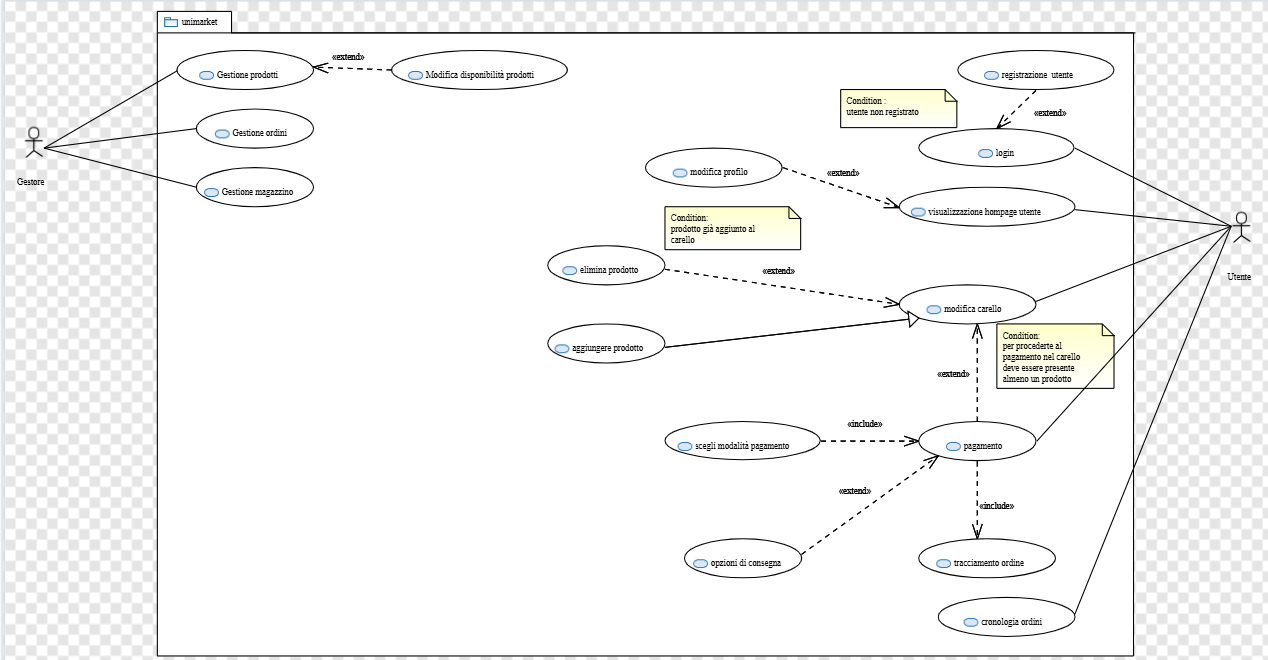
\includegraphics[width=0.8\textwidth]{../UML/UML png/UseCaseDiagram.png}
    \label{fig:Use Case Diagram}
\end{figure}
\subsubsection{Class Diagram}
Il diagramma delle classi modella le classi contenute nel sitema, con i relativi metodi e attributi.
\begin{figure}[H]
    \centering
    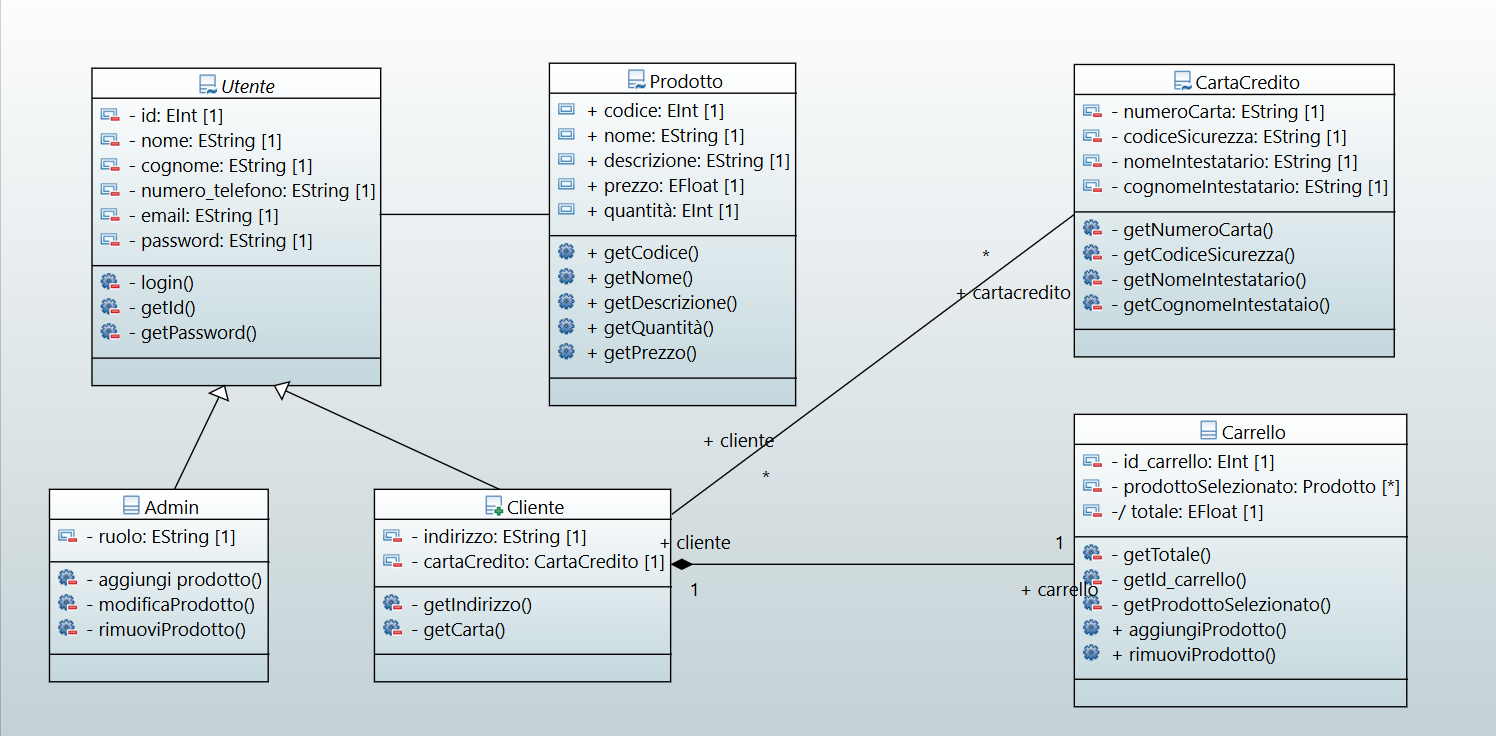
\includegraphics[width=0.8\textwidth]{../UML/UML png/ClassDiagram.png}
    \label{fig:Class Diagram}
\end{figure}
\subsubsection{State Machinne}
Il diagramma degli stati modella il comportamento di un oggetto in base allo stato in cui si trova.
Nello specifico, il seguente diagramma modella gli stati attivi durante l'utilizzo del sistema da un utente.
\begin{figure}[H]
    \centering
    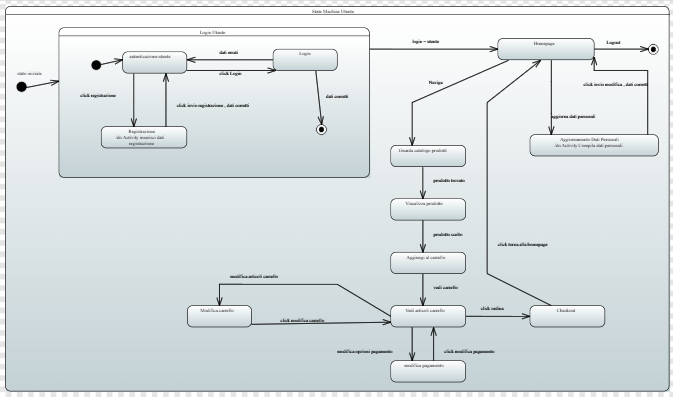
\includegraphics[width=0.8\textwidth]{../UML/UML png/StateMachine.png}
    \label{fig:State Machine}
\end{figure}
\newpage
\subsubsection{Sequence Diagram}
Il diagramma delle sequenze modella l'interazione tra gli oggetti del sistema, mostrando l'ordine in cui i messaggi vengono scambiati. Nel diagramma viene mostrata l'interazione tra l'utente e il sistema nelle operazioni di login e agiunta di prodotti al carrello.
\begin{figure}[H]
    \centering
    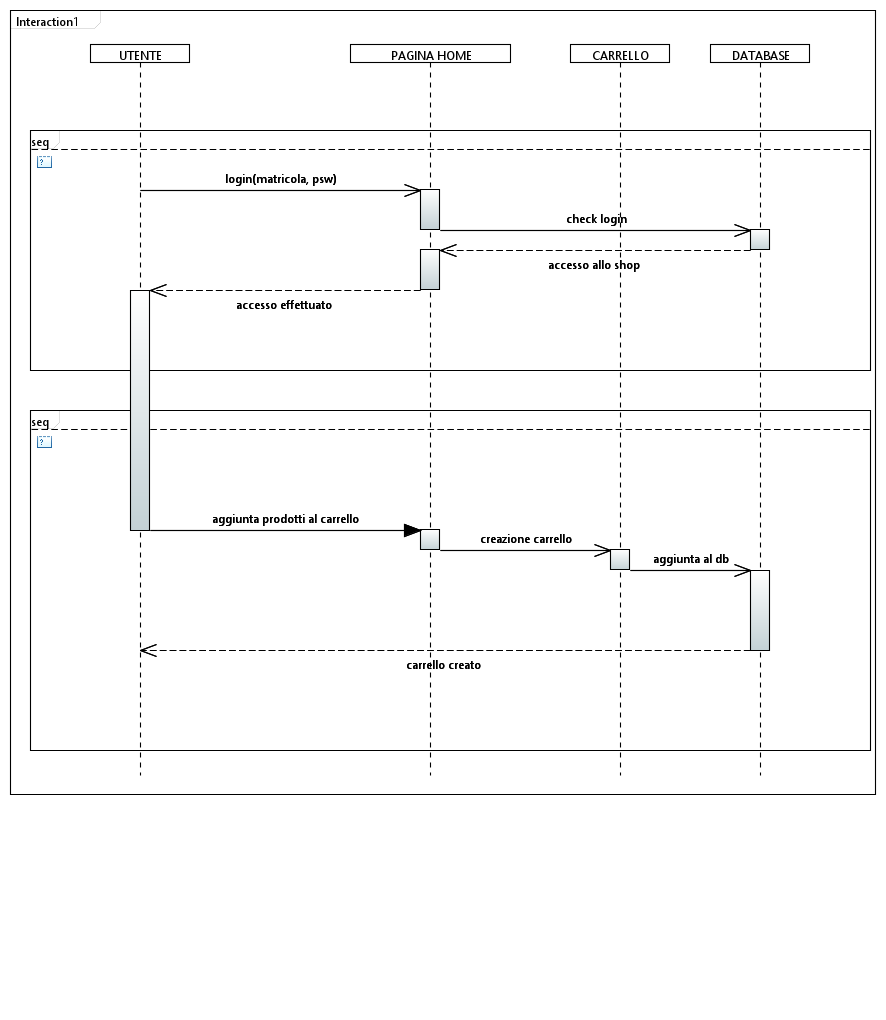
\includegraphics[width=0.8\textwidth]{../UML/UML png/Sequence_Diagram.png}
    \label{fig:Sequence Diagram}
\end{figure}
\newpage
\subsubsection{Communication Diagram}
Il diagramma di comunicazione modella lo scambio di messaggi tra le componenti del sistema durante l'aggiunta, da parte dell'utente, di prodotti al carrello.
\begin{figure}[H]
    \centering
    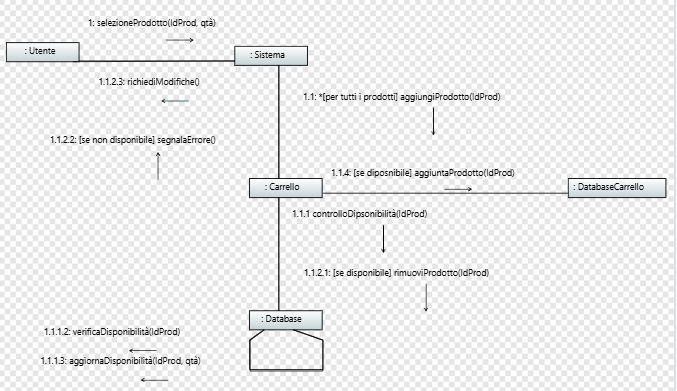
\includegraphics[width=0.8\textwidth]{../UML/UML png/CommunicationDiagram.png}
    \label{fig:Communication Diagram}
\end{figure}
\subsubsection{Activity Diagram}
Il diagramma delle attività modella il flusso di lavoro all'interno del sistema, mostrando le attività e le decisioni che vengono prese durante l'interazione con l'applicazione.   
Il diagramma seguente mostra il flusso di lavoro per l'aggiunta di un prodotto al carrello.
\begin{figure}[H]
    \centering
    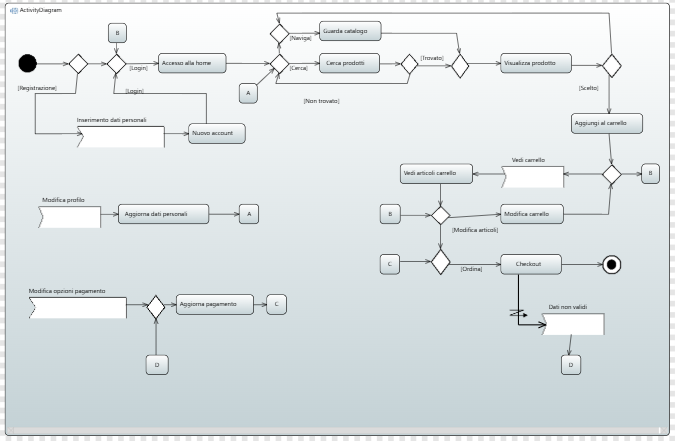
\includegraphics[width=0.8\textwidth]{../UML/UML png/ActivityDiagram.png}
    \label{fig:Activity Diagram}
\end{figure}
\textit{Nota: i connettori(A,B,C,D) sono stati rappresentati usando blocchi azione per l'assenza di un blocco dedicato da parte di Papyrus.}

\subsubsection{Component Diagram}
Il diagramma delle componenti ha lo scopo di mostrare le relazioni tra le diverse componenti di un sistema. Nel diagramma seguente vengono mostrate le relazioni tra i tre livelli del sistema.
\begin{figure}[H]
    \centering
    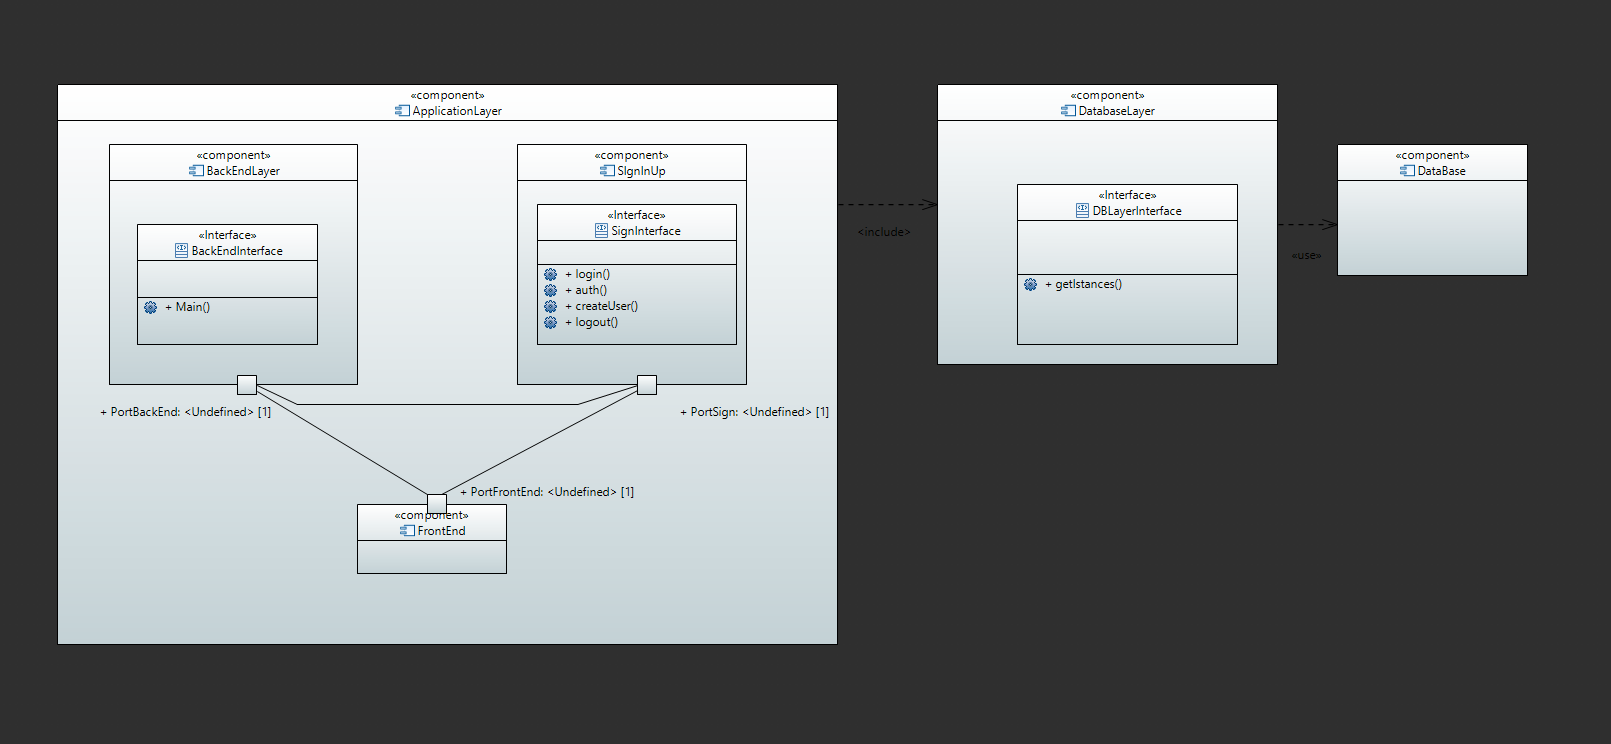
\includegraphics[width=0.8\textwidth]{../UML/UML png/diagramma dei Componenti.png}
    \label{fig:Component Diagram}
\end{figure}
\subsubsection{Package Diagram}
Il diagramma dei pacchetti mostra la struttura del programma e le interazioni tra i vari package.

Nel digramma riportato, a sinistra è il diagramma concettuale, mostra l'architettura ideata all'inizio dello sviluppo; a destra la rappresentazione effettiva delle interazioni, fornita da un'analisi effettuata con STAN.
\begin{figure}[H]
    \centering
    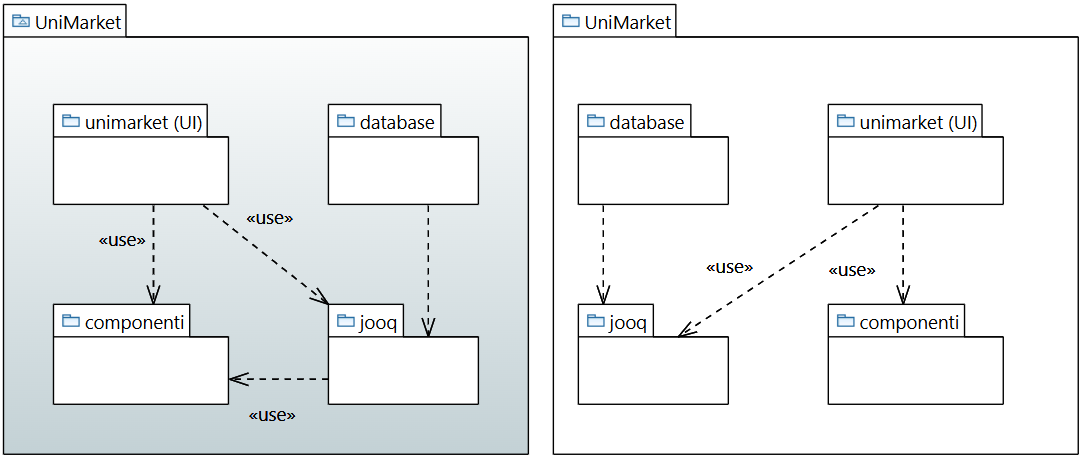
\includegraphics[width=0.8\textwidth]{../UML/UML png/PackageDiagram.png}
    \label{fig:Package Diagram}
\end{figure}
\subsection{Architettura del software}
\subsubsection{Viste architettoniche}
Le viste architettoniche e i punti di vista utilizzati sono:
\begin{itemize}
    \item \textbf{Modulo:} È stato utilizzato il punto di vista \textbf{a strati}, che permette di visualizzare il sistema su livelli, i cui elementi possono utilizzare elementi di un livello inferiore.  
    \item \textbf{Componenti e connettori:} È stato utilizzato il punto di vista \textbf{client-server}, che descrive un sistema costituito da client e server cooperanti. In questo progetto, il client rappresenta l'interfaccia utente dell'applicazione e il server gestisce la logica di business e l'accesso ai dati.
    \item \textbf{Realizzativa:} È stato utilizzato il punto di vista dell'\textbf{implementazione}, che descrive come i componenti logici e le funzionalità di alto livello vengono tradotti in strutture fisiche e tecniche. 
    \begin{itemize}
        \item Il progetto è organizzato seguendo un approccio \textbf{maven}, con una struttura standard: \textbf{src/main/java} per il codice sorgente, \textbf{src/main/resources} per le risorse, \textbf{src/test/java} per i test.
        \item I framework utilizzati sono: \textbf{Vaadin} per l'interfaccia utente, \textbf{JOOQ} per l'accesso ai dati, \textbf{SQLite} per il database.
    \end{itemize}
\end{itemize}

\subsubsection{Stile architettonico}
Il progetto è basato sullo stile architettonico a \textbf{tre livelli}, che prevede la suddivisione del sistema in tre strati distinti: livello database, livello di persistenza e livello di presentazione. Questo approccio consente di separare le funzionalità e i compiti del sistema, semplificando la gestione e la manutenzione del codice.
\begin{itemize}
    \item \textbf{Livello Database:} 
    Il livello database gestisce la memorizzazione e l'accesso ai dati, garantendo la persistenza delle informazioni. In questo progetto, è implementato un \textit{database embedded} utilizzando \textit{SQLite}.
    \item \textbf{Livello di Persistenza:} 
    Il livello di persistenza si occupa di gestire la comunicazione tra il livello database e il livello di presentazione, fornendo un'interfaccia per l'accesso ai dati. In questo progetto, il livello di persistenza è implementato utilizzando \textit{JOOQ}, un framework Java per la creazione di query SQL.   
    \item \textbf{Livello di Presentazione:} 
    Il livello di presentazione gestisce l'interfaccia utente e l'interazione con l'utente. In questo progetto, il livello di presentazione è implementato utilizzando \textit{Vaadin}, un framework Java per lo sviluppo di applicazioni web.
\end{itemize}
\subsubsection{Librerie esterne}
Il progetto utilizza diverse librerie per gestire l’interfaccia utente, il database, la persistenza dei dati e il logging. Di seguito sono descritte alcune delle più rilevanti.
\begin{itemize}
    \item \textbf{Vaadin:} Framework Java per lo sviluppo di applicazioni web, utilizzato per la creazione dell'interfaccia utente. Fornisce componenti UI reattivi e un’integrazione fluida con Spring Boot.Fornisce componenti UI reattivi e un’integrazione fluida con Spring Boot.
    \item \textbf{JOOQ:} Framework Java per la creazione di query SQL, utilizzato per la gestione della persistenza dei dati.
    \item \textbf{SQLite:} Database embedded utilizzato per la memorizzazione dei dati.
    \item \textbf{log4j e slf4j:} Framework per la gestione dei log, utilizzati per il debugging e per registrare eventi e informazioni sul funzionamento dell'applicazione.
    \item \textbf{hibernate} \textit{Object-Relational Mapping} (ORM) framework, utilizzato per la gestione della persistenza dei dati. Permette l'integrazione con Spring Data JPA per un accesso semplificato ai dati.
\end{itemize}
\subsection{Software Design}
\subsubsection{Complessità e misurazioni}
\paragraph{Analisi strutturale}\leavevmode\par

L'analisi strutturale del codice ha lo scopo di valutare la complessità e la qualità del codice sorgente, identificando eventuali punti deboli e aree di miglioramento. Questo processo include la misurazione di metriche chiave come la complessità ciclomatica, la coesione e il grado di accoppiamento tra i moduli. 

Nel progetto è stata svolta un'analisi strutturale tramite \textbf{STAN}, che permette di valutare le interazioni e dipendenze tra classi e pacchetti.
Tramite STAN è stato possibile individuare cicli interni al sistema e risolverli. 

Ad esempio:
\begin{figure}[H]
    \centering
    \begin{minipage}{0.45\textwidth}
        \centering
        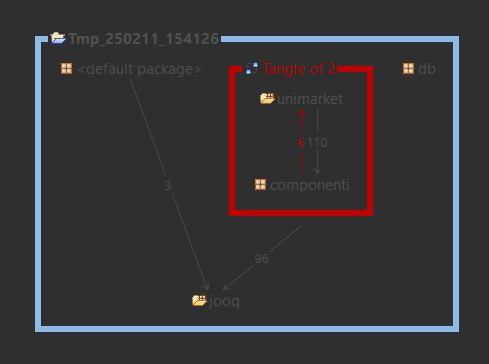
\includegraphics[width=\textwidth]{../Media/STAN/cicloPacchetti.png}
        \caption{Implementazione scorretta dei pattern}
        \label{fig:cicloPacchetti}
    \end{minipage}
    \hfill
    \begin{minipage}{0.45\textwidth}
        \centering
        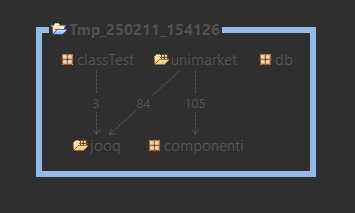
\includegraphics[width=\textwidth]{../Media/STAN/pacchetti.png}
        \caption{Pacchetti corretti}
        \label{fig:pacchetti}
    \end{minipage}
\end{figure}

L'analisi ha permesso di identificare un ciclo tra i pacchetti \textit{unimarket}, il livello di presentazione, e \textit{componenti}. 
Questo errore era causato dalla scorretta implementazione dei pattern. Una volta individuato è stato possibile correggerlo per ottenere un'interazione senza cicli:

\subsubsection{Design Patterns}

I pattern utilizzati nel progetto sono:
\begin{itemize}
    \item \textbf{Factory pattern}: Implementato tramite il servizio \textit{CarrelloService}, permette di garantire l'associazione di un carrello ad ogni utente al momento del login; se un utente ha già un carrello,  questo viene recuperato dal database, altrimenti ne viene creato uno. Permette di evitare duplicazioni, migliora la manutenibilità e separa la logica dalla gestione.
    \item \textbf{Observer pattern}: Implementato tramite due interfacce \textit{Observer}: una per la gestione e una per l'interfaccia. L'oggetto osservato è il \textit{Carrello}, tramite la gestione e notifica degli observer in \textit{CarrelloService}, permette di aggiornare in tempo reale le classi e interfacce che ne mostrano il contenuto. 
\end{itemize}

\newpage
\section{Testing}
\subsection{Testing e Verifica del Sistema}
Durante il ciclo di vita del progetto, oltre allo sviluppo del codice e alla scrittura della documentazione, un ruolo fondamentale è stato svolto dalla fase di testing. L'obiettivo principale è stato garantire la correttezza e l'affidabilità del sistema, prevenendo errori e malfunzionamenti che avrebbero potuto comprometterne l’utilizzo.

È noto che molti problemi emergono nelle prime fasi dello sviluppo software, ma se individuati in ritardo possono risultare più complessi e costosi da correggere. Per questo motivo, il testing è stato integrato sin dalle prime fasi del progetto, adottando un approccio progressivo e iterativo.

\subsection{Testing in fase di sviluppo}
La prima fase del testing è avvenuta in parallelo con la scrittura del codice. Per verificare il corretto funzionamento delle funzionalità integrate, sono stati adottati strumenti di logging e controlli temporanei, facilitando il debugging e l’individuazione tempestiva di errori. Il controllo è stato eseguito manualmente, testando direttamente le funzionalità con valori di input specifici e verificando il comportamento del sistema tramite i log di esecuzione.

\subsection{Testing automatizzato}
Per garantire una maggiore copertura del sistema e validare il corretto funzionamento delle diverse componenti, è prevista l'implementazione di test automatici. L'obiettivo è scrivere test unitari e di integrazione che verifichino il comportamento del codice in modo sistematico. Tuttavia, per ragioni di tempistiche, questa fase è stata parzialmente posticipata e non è ancora completamente integrata nel processo di sviluppo.

L'implementazione dei test automatici avviene all'interno della directory \textit{src/test/java} utilizzando JUnit, un framework per il testing unitario in Java. I test vengono scritti per verificare il corretto funzionamento dei metodi e delle classi, simulando l'input e confrontando l'output con quello atteso.

Un esempio di test automatico implementato è la classe di test \textit{CartaServiceTest}, che verifica il metodo \textit{salvaCarta}. Questo metodo si occupa di inserire nel database un nuovo oggetto \textit{CartaCredito}, salvando i dati del numero di carta, codice di sicurezza e intestatario. Il test controlla che l'inserimento avvenga correttamente e gestisce eventuali errori di persistenza.

\newpage
\section{Maintenance}
\subsection{Manutenzione del Software}

La manutenzione del software comprende diverse attività mirate a garantire il corretto funzionamento del sistema nel tempo, migliorandone stabilità, efficienza e adattabilità. Si suddivide in quattro categorie principali:

\begin{enumerate}
    \item \textbf{Manutenzione correttiva}:  riguarda la risoluzione di bug e malfunzionamenti emersi durante lo sviluppo, come incompatibilità tra i tipi di dati gestiti da Java e quelli supportati dal database.
    
    \item \textbf{Manutenzione adattiva}: consiste nell'aggiornamento del software per adeguarlo a cambiamenti tecnologici o nuove esigenze operative. Pur non essendo ancora necessaria in questa fase, potenziali interventi futuri potrebbero includere l'ottimizzazione delle prestazioni, l'aggiornamento delle librerie o l'adattamento a nuove piattaforme.
    
    \item \textbf{Manutenzione perfettiva}: si concentra sul miglioramento delle funzionalità esistenti e sull'introduzione di nuove feature per ottimizzare l'interazione con il sistema.
    
    \item \textbf{Manutenzione preventiva}: ha l'obiettivo di ridurre il rischio di problemi futuri attraverso verifiche periodiche, mantenendo test e log aggiornati per semplificare la gestione del software senza complicarne inutilmente la struttura.
    
\end{enumerate}
\subsection{Best Practices}
Per garantire una manutenzione efficace e prevenire problemi derivanti da codice disorganizzato o documentazione insufficiente, sono state seguite le seguenti linee guida:
\begin{itemize}
    \item \textbf{Commenti e documentazione}:Commentare il codice per facilitarne la comprensione e la futura modificabilità.
    \item \textbf{Versionamento}: Utilizzare un sistema di versionamento per tenere traccia delle modifiche e facilitare il rollback in caso di errori.
    \item \textbf{Revisione}: Sottoporre le modifiche alla revisione del team per migliorare la qualità del codice e ridurre il rischio di errori.
    \item \textbf{Layering}: Strutturare il codice in moduli e servizi distinti, favorendo la separazione delle responsabilità e semplificando eventuali interventi futuri.
\end{itemize}
Queste attività permettono di mantenere un software facilmente gestibile e modificabile, riducendo il rischio di errori e semplificando la manutenzione nel tempo.

\subsection{Refactoring}
Il refactoring non è stato concentrato in una singola fase, ma è stato integrato durante tutto il processo di sviluppo con modifiche graduali per garantire un codice più leggibile e manutenibile. Ogni intervento ha interessato sezioni specifiche del sistema, riducendo il rischio di conflitti e garantendo il funzionamento complessivo.

Un'area chiave di intervento è stata l'ottimizzazione del codice autogenerato da Vaadin, inizialmente disordinato e poco comprensibile. È stata migliorata la struttura delle classi, separando le responsabilità e rendendo il codice più chiaro e facile da mantenere.

Altri interventi hanno riguardato la gestione dell’interfaccia utente, con particolare attenzione al flusso di navigazione, al sistema di login e alle interfacce riservate agli amministratori per il controllo dei dati salvati.
\subsection{migliorameti futuri}
Alcune funzionalità non sono ancora state implementate, ma potrebbero rappresentare possibili sviluppi futuri per arricchire il sistema. Tra queste:

\begin{itemize}
    \item \textbf{Gestione dei prodotti}: migliorare la gestione dei prodotti da parte degli amministratori, con la possibilitià di modificarne i dettagli.
    \item \textbf{Logout}: fornire l'opzione di logout per poter cambiare account.
    \item \textbf{Modificabilità account}: permettere agli utenti di eliminare il proprio account o modificare i dati salvati.
\end{itemize}
L'integrazione di queste funzionalità potrà migliorare ulteriormente l'esperienza d'uso del sistema.
\newpage
\begin{center}
\Huge \textbf{Calendario Timebox}
\end{center}

\begin{center}
\begin{tabular}{|c|c|c|}
\hline
\textbf{SETTIMANA/E} & \textbf{OBIETTIVO} & \textbf{INCONTRI } \\
\hline
4/11/2024 - 17/11/2024 & Project Plan & 6 \\
\hline
18/11/2024 - 24/11/2024 & Documentazione, gestione del progetto & 3 \\
\hline
25/11/2024 - 29/11/2024 & Documentazione, Specifica dei requisiti  & 3 \\
\hline
2/12/2024 - 5/2/2025 & UML & 2 \\
\hline
6/1/2025 - 26/1/2025 & Database, documentazione & 1 \\
\hline
27/1/2025 - 2/2/2025 & Interfaccia & 2 \\
\hline
3/2/2025 - 11/2/2025 & Interfaccia, manutenzione, documentazione & 6 \\
\hline


\end{tabular}
\end{center}

\end{document}
